\chapter{Fundamentos de programación}
\label{fundamentos-de-programaciuxf3n}


\section{Estructura de un programa}\label{estructura-de-un-programa}

Un programa es un conjunto de instrucciones codificadas que una
computadora puede ejecutar para realizar una tarea específica o resolver
un problema.

\begin{definition}[Algoritmo]
Formalmente definimos un algoritmo como un conjunto de pasos,
procedimientos o acciones que nos permiten alcanzar un resultado o
resolver un problema.  
\end{definition}

Los programas están escritos en lenguajes de programación y son creados
por programadores. Los programas pueden variar en complejidad, desde
simples scripts que realizan una acción básica hasta sistemas operativos
completos que gestionan los recursos de una computadora.


\section{Lenguajes de programación}\label{lenguajes-de-programaciuxf3n}

Un lenguaje de programación es un sistema formal diseñado para expresar
instrucciones que una computadora puede interpretar y ejecutar. Estos
lenguajes permiten a los programadores escribir programas que realizan
tareas específicas, desde operaciones simples hasta aplicaciones
complejas. Los lenguajes de programación proporcionan una manera de
comunicarse con la computadora utilizando una sintaxis y semántica
específica.

Algunas características clave de los lenguajes de programación incluyen:

\begin{itemize}
  \item \textbf{Sintaxis}: El conjunto de reglas que define cómo se deben
    escribir las instrucciones y declaraciones en el lenguaje.
  \item \textbf{Semántica}: El significado de las instrucciones escritas en el
    lenguaje.
  \item \textbf{Abstracción}: La capacidad de definir estructuras y
    operaciones de alto nivel que oculten detalles complejos.
  \item \textbf{Paradigmas}: Los enfoques o estilos de programación que el
    lenguaje soporta, como la programación estructurada, la programación
    orientada a objetos, la programación funcional, entre otros.
\end{itemize}

Existen muchos lenguajes de programación, cada uno con sus propias
características y propósitos. Algunos ejemplos comunes incluyen:

\begin{itemize}
\item
  \textbf{Python}: Conocido por su sintaxis clara y legible, es
  ampliamente utilizado en ciencia de datos, desarrollo web,
  automatización y más.
\item
  \textbf{Java}: Utilizado en desarrollo de aplicaciones empresariales,
  aplicaciones móviles y sistemas integrados.
\item
  \textbf{C}: Un lenguaje de bajo nivel que proporciona control
  detallado sobre el hardware de la computadora, utilizado en sistemas
  operativos y software de sistemas.
\item
  \textbf{JavaScript}: Utilizado principalmente en el desarrollo web
  para crear aplicaciones interactivas y dinámicas.
\item
  \textbf{Ruby}: Conocido por su simplicidad y elegancia, utilizado en
  desarrollo web y automatización.
\end{itemize}

Cada lenguaje de programación está diseñado con ciertos objetivos en
mente y puede ser más adecuado para ciertos tipos de tareas o proyectos.

\subsection{Los lenguajes de programación más
utilizados}\label{los-lenguajes-de-programactightlistiuxf3n-muxe1s-utilizados}

En la figura \ref{fig:lenguajesDemandados} se muestran los lenguajes de programación con 
mayor demanda en el 2023.

\begin{figure}
  \centering
  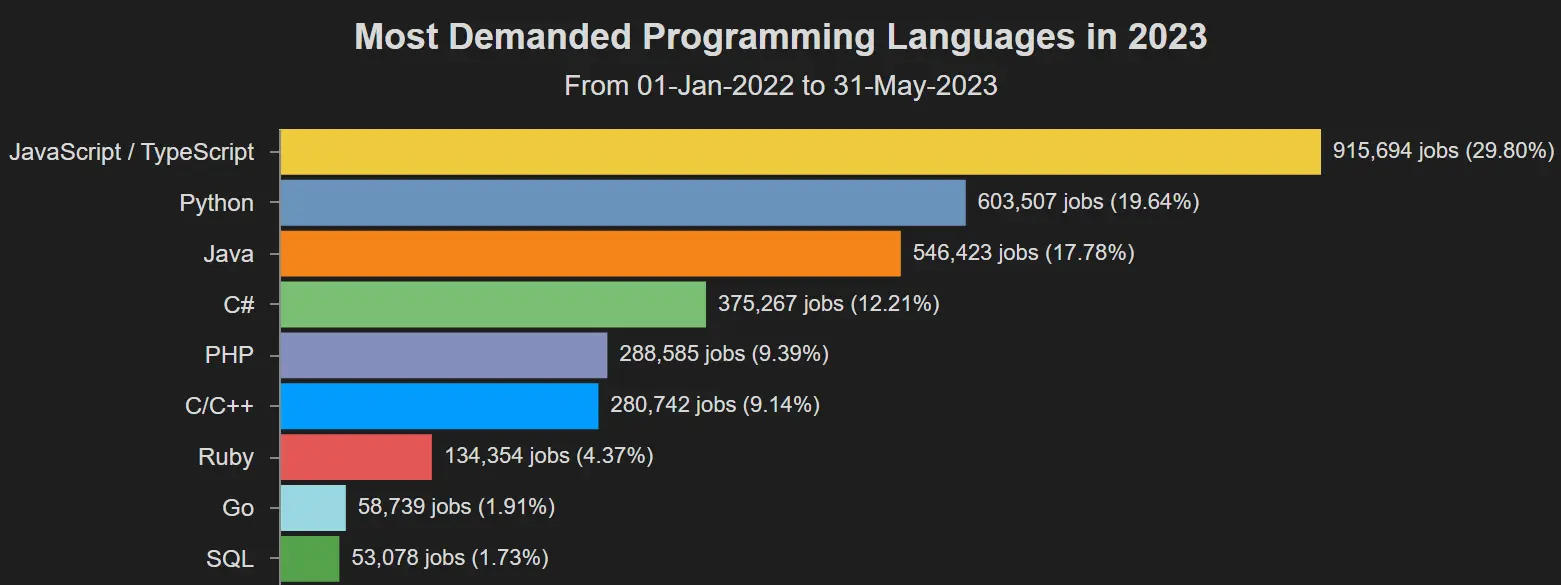
\includegraphics[keepaspectratio]{img/lenguajes.png}
  \caption{Lenguajes más demandados en 2023}
  \label{fig:lenguajesDemandados}
\end{figure}


\section{Lenguajes interpretados y compilados}\label{lenguajes-interpretados-y-compilados}

La principal diferencia entre los lenguajes de programación compilados y
los interpretados radica en cómo se ejecutan las instrucciones del
programa:

\subsection{Lenguajes de Programación Compilados}\label{lenguajes-de-programaciuxf3n-compilados}

\begin{enumerate}
  \item Proceso de Compilación: 
    \begin{itemize}
      \item
        Compilador: Un compilador traduce el código fuente completo a código
        máquina o bytecode antes de que el programa se ejecute. Este proceso
        se realiza una sola vez y genera un archivo ejecutable independiente.
      \item
        Ejemplo: C, C++, Rust, Go.
      \end{itemize}

  \item Ventajas:
      \begin{itemize}
        \item
          Rendimiento: Los programas compilados suelen ejecutarse más rápido que
          los interpretados porque la traducción a código máquina se realiza una
          sola vez y el ejecutable resultante está optimizado.
        \item
          Optimización: Los compiladores pueden realizar optimizaciones
          avanzadas durante la compilación para mejorar la eficiencia del
          programa.
      \end{itemize}

  \item Desventajas:
      \begin{itemize}
        \item
          Tiempo de Compilación: El proceso de compilación puede ser lento,
          especialmente para programas grandes.
        \item
          Portabilidad: El código compilado suele estar ligado a una plataforma
          específica, lo que puede dificultar su portabilidad a diferentes
          sistemas operativos.
      \end{itemize}
\end{enumerate}

\subsection{Lenguajes de Programación Interpretados}\label{lenguajes-de-programaciuxf3n-interpretados}

\begin{enumerate}
  \item Proceso de Interpretación:
    \begin{itemize}
      \item
        Intérprete: Un intérprete traduce y ejecuta el código fuente línea por
        línea en tiempo de ejecución, sin generar un archivo ejecutable
        intermedio.
      \item
        Ejemplo: Python, JavaScript, Ruby, PHP.
    \end{itemize}
  \item Ventajas:
    \begin{itemize}
      \item
        Desarrollo Rápido: No es necesario compilar el código antes de
        ejecutarlo, lo que permite ciclos de desarrollo y pruebas más rápidos.
      \item
        Portabilidad: Los programas interpretados pueden ejecutarse en
        cualquier plataforma que tenga el intérprete adecuado, lo que mejora
        su portabilidad.
    \end{itemize}

  \item Desventajas:
    \begin{itemize}
      \item
        Rendimiento: Los programas interpretados suelen ser más lentos que los
        compilados porque la traducción a código máquina ocurre en tiempo de
        ejecución.
      \item
        Optimización: Las oportunidades de optimización en tiempo de ejecución
        son limitadas en comparación con la compilación previa.
    \end{itemize}
  
\end{enumerate}


\subsection{Ejemplos y Consideraciones}\label{ejemplos-y-consideraciones}

\begin{description}
\item[Java:] Es un caso interesante porque utiliza un enfoque mixto. El
  código Java se compila en bytecode, que es interpretado por la Máquina
  Virtual de Java (JVM). Además, la JVM utiliza un compilador JIT
  (Just-In-Time) para convertir partes del bytecode en código máquina
  durante la ejecución, combinando ventajas de ambos enfoques.
\item[Python:] Aunque es principalmente un lenguaje interpretado, también
  puede ser compilado a bytecode (.pyc) para ser ejecutado por la
  máquina virtual de Python, lo que mejora ligeramente su rendimiento,
  pero no alcanza la velocidad de un lenguaje completamente compilado
  como C++.
\end{description}

En conclusión, la elección entre un lenguaje compilado y uno
interpretado depende de varios factores, incluyendo la necesidad de
rendimiento, la rapidez del desarrollo, y la portabilidad del código.

\section{Python}\label{python}

\subsection{¿Qué es Python?}\label{quuxe9-es-python}

Python es un lenguaje de programación popular. Fue creado por Guido van
Rossum y lanzado en 1991.

Se utiliza para:

\begin{itemize}
  \item Desarrollo web (del lado del servidor),
  \item Desarrollo de software,
  \item Matemáticas,
  \item Inteligencia Artificial,
  \item Scripting.
\end{itemize}

\subsection{¿Qué puede hacer Python?}\label{quuxe9-puede-hacer-python}

\begin{itemize}
  \item Python se puede utilizar en un servidor para crear aplicaciones web.
  \item Python se puede utilizar junto con el software para crear flujos de trabajo.
  \item Python puede conectarse a sistemas de bases de datos. También puede
    leer y modificar archivos.
  \item Python se puede utilizar para manejar Big Data y realizar matemáticas
    complejas.
  \item Python se puede utilizar para la creación rápida de prototipos o para
    el desarrollo de software listo para producción.
\end{itemize}

\subsection{¿Por qué Python?}\label{por-quuxe9-python}

\begin{itemize}
  \item Python funciona en diferentes plataformas (Windows, Mac, Linux,
    Raspberry Pi, etc.).
  \item Python tiene una sintaxis simple similar a la del idioma inglés.
  \item Python tiene una sintaxis que permite a los desarrolladores escribir
    programas con menos líneas que otros lenguajes de programación.
  \item Python se ejecuta en un sistema de interpretación, lo que significa
    que el código se puede ejecutar tan pronto como se escribe. Esto
    significa que la creación de prototipos puede ser muy rápida.
  \item Python se puede tratar de forma procedimental, orientada a objetos o
    funcional.
\end{itemize}

\subsection{Es bueno saber}\label{es-bueno-saber}

\begin{itemize}
\item
  La versión principal más reciente de Python es Python 3, que usaremos
  en este curso. Sin embargo, Python 2, aunque no se actualiza con nada
  más que actualizaciones de seguridad, sigue siendo bastante popular.
\item
  En este curso, Python se escribirá en un editor de texto. Es posible
  escribir Python en un entorno de desarrollo integrado, como Thonny,
  Pycharm, Visual Studio Code, Google Colaboratory, Netbeans o Eclipse,
  que son particularmente útiles cuando se administran colecciones más
  grandes de archivos Python.
\end{itemize}

\subsection{Sintaxis de Python comparada con otros lenguajes de
programación}\label{sintaxis-de-python-comparada-con-otros-lenguajes-de-programaciuxf3n}

\begin{itemize}
\item
  Python fue diseñado para facilitar la lectura y tiene algunas
  similitudes con el idioma inglés con influencia de las matemáticas.
\item
  Python usa nuevas líneas para completar un comando, a diferencia de
  otros lenguajes de programación que suelen usar punto y coma o
  paréntesis.
\item
  Python se basa en la sangría, utilizando espacios en blanco, para
  definir el alcance; como el alcance de los bucles, funciones y clases.
  Otros lenguajes de programación suelen utilizar llaves para este
  propósito.
\end{itemize}

\subsection{Instalación de Python}\label{instalaciuxf3n-de-python}

Muchas PC y Mac ya tienen Python instalado.

Para comprobar si tiene Python instalado en una PC con Windows, busque
Python en la barra de inicio o ejecute lo siguiente en la línea de
comandos (cmd.exe):

\begin{verbatim}
C:\Usuarios\Su nombre>python --version
\end{verbatim}

Para verificar si tiene Python instalado en Linux o Mac, en Linux abra
la línea de comando o en Mac abra la Terminal y escriba:

\begin{verbatim}
python --versión
\end{verbatim}

Si descubre que no tiene Python instalado en su computadora, puede
descargarlo de forma gratuita desde el siguiente sitio web:
\url{https://www.python.org/}

\subsection{Mi primer programa en Python}\label{mi-primer-programa-en-python}

\begin{Shaded}
\begin{Highlighting}[]
\BuiltInTok{print}\NormalTok{(}\StringTok{"Hola mundo"}\NormalTok{)}
\end{Highlighting}
\end{Shaded}

\section{Funciones}\label{funciones}

Una función es un bloque de código que sólo se ejecuta cuando se llama.
Puede pasar datos, conocidos como parámetros, a una función. Una función
puede devolver datos como resultado.

\subsection{Declarar una función}\label{declarar-una-funciuxf3n}

En Python una función se define usando la palabra clave \texttt{def}:

\begin{Shaded}
\begin{Highlighting}[]
\KeywordTok{def}\NormalTok{ mi\_función():}
    \BuiltInTok{print}\NormalTok{(}\StringTok{"Hola desde una función"}\NormalTok{)}
\end{Highlighting}
\end{Shaded}

\subsection{Llamar a una función}\label{llamar-a-una-funciuxf3n}

Para llamar a una función, use el nombre de la función seguido de
paréntesis:

\begin{Shaded}
\begin{Highlighting}[]
\KeywordTok{def}\NormalTok{ mi\_función():}
    \BuiltInTok{print}\NormalTok{(}\StringTok{"Hola desde una función"}\NormalTok{)}

\NormalTok{mi\_función()}
\end{Highlighting}
\end{Shaded}

\subsection{Argumentos}\label{argumentos}

La información se puede pasar a funciones como argumentos. Los
argumentos se especifican después del nombre de la función, dentro del
paréntesis. Puedes agregar tantos argumentos como quieras, simplemente
sepáralos con una coma.

El siguiente ejemplo tiene una función con un argumento (fname). Cuando
se llama a la función, pasamos un nombre, que se usa dentro de la
función para imprimir el nombre completo:

\begin{Shaded}
\begin{Highlighting}[]
\KeywordTok{def}\NormalTok{ mi\_función(fname):}
    \BuiltInTok{print}\NormalTok{(fnombre }\OperatorTok{+} \StringTok{" Refsnes"}\NormalTok{)}

\NormalTok{mi\_funcion(}\StringTok{"Emil"}\NormalTok{)}
\NormalTok{mi\_función(}\StringTok{"Tobías"}\NormalTok{)}
\NormalTok{mi\_función(}\StringTok{"Linus"}\NormalTok{)}
\end{Highlighting}
\end{Shaded}

\subsection{Argumentos arbitrarios,
*args}\label{argumentos-arbitrarios-args}

Si no sabe cuántos argumentos se pasarán a su función, agregue un
\_\_*\_\_ antes del nombre del parámetro en la definición de la función.
De esta manera, la función recibirá una tupla de argumentos y podrá
acceder a los elementos en consecuencia:

\begin{Shaded}
\begin{Highlighting}[]
\KeywordTok{def}\NormalTok{ mi\_funcion(}\OperatorTok{*}\NormalTok{ninos):}
    \BuiltInTok{print}\NormalTok{(}\StringTok{"El hijo menor es "} \OperatorTok{+}\NormalTok{ ninos[}\DecValTok{2}\NormalTok{])}

\NormalTok{mi\_funcion(}\StringTok{"Emil"}\NormalTok{, }\StringTok{"Tobías"}\NormalTok{, }\StringTok{"Linus"}\NormalTok{)}
\end{Highlighting}
\end{Shaded}

\section{Módulos de Python}\label{muxf3dulos-de-python}

\subsection{¿Qué es un módulo?}\label{quuxe9-es-un-muxf3dulo}

Considere que un módulo es lo mismo que una biblioteca de código. Un
archivo que contiene un conjunto de funciones que desea incluir en su
aplicación.

\subsection{Crear un módulo}\label{crear-un-muxf3dulo}

Para crear un módulo simplemente guarde el código que desea en un
archivo con la extensión de archivo \texttt{.py}:

\textbf{Ejemplo} Guarde este código en un archivo
\texttt{llamadomymodule.py}

\begin{Shaded}
\begin{Highlighting}[]
\KeywordTok{def}\NormalTok{ greeting(name):}
    \BuiltInTok{print}\NormalTok{(}\StringTok{"Hello, "} \OperatorTok{+}\NormalTok{ name)}
\end{Highlighting}
\end{Shaded}

\subsection{Utilice un módulo}\label{utilice-un-muxf3dulo}

Ahora podemos utilizar el módulo que acabamos de crear, mediante la
importdeclaración: \textbf{Ejemplo} Importa el módulo llamado mymodule y
llama a la función de saludo:

\begin{Shaded}
\begin{Highlighting}[]
    \ImportTok{import}\NormalTok{ mymodule}

\NormalTok{    mymodule.greeting(}\StringTok{"Jonathan"}\NormalTok{)}
\end{Highlighting}
\end{Shaded}

\subsection{Variables en el módulo}\label{variables-en-el-muxf3dulo}

El módulo puede contener funciones, como ya se ha descrito, pero también
variables de todo tipo (matrices, diccionarios, objetos, etc.):

\textbf{Ejemplo} Guarda este código en el \texttt{archivomymodule.py}

\begin{Shaded}
\begin{Highlighting}[]
\NormalTok{person1 }\OperatorTok{=}\NormalTok{ \{}
    \StringTok{"name"}\NormalTok{: }\StringTok{"John"}\NormalTok{,}
    \StringTok{"age"}\NormalTok{: }\DecValTok{36}\NormalTok{,}
    \StringTok{"country"}\NormalTok{: }\StringTok{"Norway"}
\NormalTok{\}}
\end{Highlighting}
\end{Shaded}

\textbf{Ejemplo} Importe el módulo llamado \texttt{mymodule} y acceda al
diccionario \texttt{person1}:

\begin{Shaded}
\begin{Highlighting}[]
    \ImportTok{import}\NormalTok{ mymodule}

\NormalTok{    a }\OperatorTok{=}\NormalTok{ mymodule.person1[}\StringTok{"age"}\NormalTok{]}
    \BuiltInTok{print}\NormalTok{(a)}
\end{Highlighting}
\end{Shaded}

\subsection{Nombrar un módulo}\label{nombrar-un-muxf3dulo}

Puedes nombrar el archivo del módulo como quieras, pero debe tener la
extensión de archivo \texttt{.py}

\subsection{Cambiar el nombre de un
módulo}\label{cambiar-el-nombre-de-un-muxf3dulo}

Puedes crear un alias al importar un módulo, utilizando la aspalabra
clave:

\textbf{Ejemplo} Crear un alias para mymoduleel llamado \texttt{mx}:

\begin{Shaded}
\begin{Highlighting}[]
\ImportTok{import}\NormalTok{ mymodule }\ImportTok{as}\NormalTok{ mx}

\NormalTok{a }\OperatorTok{=}\NormalTok{ mx.person1[}\StringTok{"age"}\NormalTok{]}
\BuiltInTok{print}\NormalTok{(a)}
\end{Highlighting}
\end{Shaded}

\subsection{Módulos integrados}\label{muxf3dulos-integrados}

Hay varios módulos integrados en Python que puedes importar cuando
quieras.

\textbf{Ejemplo} Importar y utilizar el \texttt{platformmódulo}:

\begin{Shaded}
\begin{Highlighting}[]
\ImportTok{import}\NormalTok{ platform}

\NormalTok{x }\OperatorTok{=}\NormalTok{ platform.system()}
\BuiltInTok{print}\NormalTok{(x)}
\end{Highlighting}
\end{Shaded}

\subsection{Usando la función dir()}\label{usando-la-funciuxf3n-dir}

Hay una función incorporada para enumerar todos los nombres de funciones
(o nombres de variables) en un módulo. La función \texttt{dir()}:

\textbf{Ejemplo} Enumere todos los nombres definidos que pertenecen al
módulo de la plataforma:

\begin{Shaded}
\begin{Highlighting}[]
\ImportTok{import}\NormalTok{ platform}

\NormalTok{x }\OperatorTok{=} \BuiltInTok{dir}\NormalTok{(platform)}
\BuiltInTok{print}\NormalTok{(x)}
\end{Highlighting}
\end{Shaded}

\subsection{Importar desde módulo}\label{importar-desde-muxf3dulo}

Puede elegir importar solo partes de un módulo, utilizando la
frompalabra clave.

\textbf{Ejemplo} El módulo nombrado \texttt{mymodule} tiene una función
y un diccionario:

\begin{Shaded}
\begin{Highlighting}[]
\KeywordTok{def}\NormalTok{ greeting(name):}
    \BuiltInTok{print}\NormalTok{(}\StringTok{"Hello, "} \OperatorTok{+}\NormalTok{ name)}

\NormalTok{person1 }\OperatorTok{=}\NormalTok{ \{}
    \StringTok{"name"}\NormalTok{: }\StringTok{"John"}\NormalTok{,}
    \StringTok{"age"}\NormalTok{: }\DecValTok{36}\NormalTok{,}
    \StringTok{"country"}\NormalTok{: }\StringTok{"Norway"}
\NormalTok{\}}
\end{Highlighting}
\end{Shaded}

\textbf{Ejemplo} Importe únicamente el diccionario \texttt{person1} del
módulo:

\begin{Shaded}
\begin{Highlighting}[]
\ImportTok{from}\NormalTok{ mymodule }\ImportTok{import}\NormalTok{ person1}

\BuiltInTok{print}\NormalTok{ (person1[}\StringTok{"age"}\NormalTok{])}
\end{Highlighting}
\end{Shaded}

\section{Referencias}

\begin{itemize}
\tightlist
\item
  \href{https://www.w3schools.com/python/}{Python en la W3Schools}
\item
  \href{https://www.python.org/}{Python.org}
\item
  \href{https://chatgpt.com/}{chatGPT en openAI}
\item
  \href{https://lab.anahuac.mx/~hselley/ayp/conceptosBasicos.html}{Algoritmos
  y Programación}
\item
  \href{https://lab.anahuac.mx/~hselley/mn/python.html}{Sintaxis básica
  en Python}
\end{itemize}
